\documentclass[../Main.tex]{subfiles}
\begin{document}

\section{Problem}
\label{sec:problem}

Today, as society continues to develop, many workers and students are moving away from home to work or study, making it crucial to find accommodation near their workplace or school.
Not every work area or school has enough dormitories for workers or students, especially during hot, rainy, or cold days, which causes inconvenience and difficulty in finding rental rooms, particularly for students and even for working individuals.

Information technology, and especially the Internet, has transformed the way people live, communicate, work, and access diverse and fast information sources.
The advent of the Internet has become a powerful tool for those looking for resources in general or searching for rental rooms in particular, making it easier than ever.
For those in need of renting accommodation, traditional search methods can be challenging, time-consuming, and labor-intensive to find rooms that meet their criteria.
For landlords, reaching potential tenants is quite challenging due to location and limited communication methods.
Now, with the advent of network systems, just a computer connected to the internet allows us to post and search for rental rooms anywhere, with prices suitable to our needs easily.

From these reasons, I decided to choose the topic ``Building a website to Finding Rental Rooms''.
With the desire to create a website that supports users in posting and searching for rental rooms that match their needs.

\section{Purpose and requirements}
\label{sec:purpose}

\subsection{Purpose}

Currently, there are many websites and applications on the internet that help users search for and post rental listings, such as phongtro123.com, nhatot.com, and ohanaliving.vn.
While these websites generally meet the functional requirements of a rental search platform, they share a common issue: the cost of posting listings is too high.
Landlords have to pay a significant fee to list their rentals on these websites.

Based on the user need for posting and searching for rental information, I propose a solution: building a website to support rental searches.
This website will enable landlords to post their rental listings at a very low cost and allow those seeking rentals to search for rooms for free.
The website will cater to the majority of users looking for rental accommodations today.
Additionally, the website will provide functionalities for administrators to manage all system information, such as user accounts, rental listings, and revenue.
It will also offer landlords features such as posting listings, managing rooms, and managing posts.

The rental search website will provide a large amount of information about houses and rooms available for rent.
Visitors to the site can use search functions to find rentals by area, such as city or district, by specific address, by rental price, and by amenities offered.

Furthermore, the website will provide detailed information about the available rentals, including addresses, email contacts, and phone numbers, allowing users to contact landlords directly.

\subsection{Requirements}

\begin{itemize}
    \item Develop a simple, user-friendly interface that is easy to use.
    \item Research and understand the essential information needed for a rental listing.
    \item Gather requirements from real users to determine what information they need about a rental room.
    \item Clearly specify requirements.
    \item Design the system specification using an object-oriented approach for easy development.
    \item Implement the system using a RESTful API approach to facilitate easy upgrades and maintenance when issues arise.
    \item Build a complete website with all necessary features.
\end{itemize}

\section{Research situations}
\label{section:research}

Renting accommodation has always been a perennial issue.
Every year, hundreds of thousands of students from various provinces across the country come to study at universities, colleges, and vocational schools.
Additionally, many employees working far from home also need to rent houses or rooms.
However, the dormitory facilities at schools or companies can only meet the needs of less than 10\% of the students and employees.
The remaining students and employees have to face the challenge of finding rental accommodation near their study or work areas, which are often very expensive and do not meet the required quantity or quality of living conditions.

Hanoi is one of the cities with the highest density of universities in the country, attracting tens of thousands of students from all over to study.
Although many universities have their own dormitories and the city has student housing, not all students qualify to live there.
Additionally, some students, either because they have the financial means or because they want to live more comfortably and not be constrained by dormitory regulations, choose to seek off-campus housing.

With the significant increase in the number of students, the demand for rental accommodation in Hanoi is rising, making the student rental market extremely dynamic and competitive.
This has led to a shortage of available rentals and fierce price competition among landlords.
As a new academic year approaches, rental prices in areas near top universities are significantly higher compared to other areas.
One of the main challenges for students in finding rental accommodation is the quality and amenities of the rooms.
Due to high demand, many rental properties fail to meet the standards for security, hygiene, fire safety, and basic amenities.
Students often have to compromise between affordable rent and quality of living conditions.

In January 2024, Vietnam had a total of 78.44 million Internet users, with an Internet penetration rate of 79.1\% of the total population.
Analysis by Kepios indicates that the number of Internet users in Vietnam increased by an additional 502 thousand (+0.6\%) from January 2023 to January 2024.
This growth underscores the increasing number of Internet users, leading to a higher demand for accessing rental accommodation information.
Therefore, using websites to search for rental accommodations has completely replaced traditional methods, which is entirely reasonable and aligned with current trends.

Some websites support finding accommodations in Vietnam:

\begin{itemize}
    \item Website phongtro123.com
          \begin{figure}[H]
              \centering
              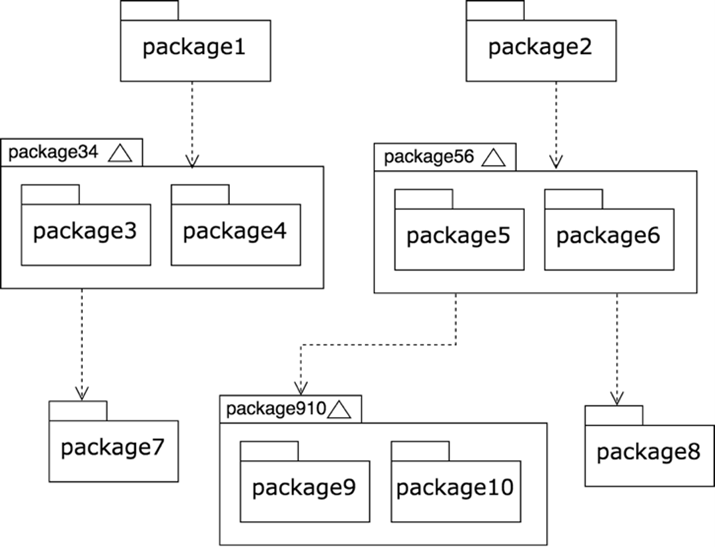
\includegraphics[width=\textwidth]{Figure/Picture1.png}
              \caption{Website phongtro123.com}
              \label{fig:phongtro123}
          \end{figure}
    \item Website nhatot.com
          \begin{figure}[H]
              \centering
              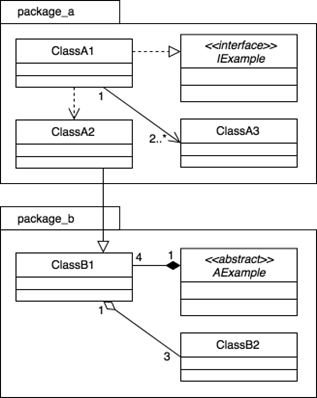
\includegraphics[width=\textwidth]{Figure/Picture2.png}
              \caption{Website nhatot.com}
              \label{fig:nhatot}
          \end{figure}
    \item Website ohanaliving.vn
          \begin{figure}[H]
              \centering
              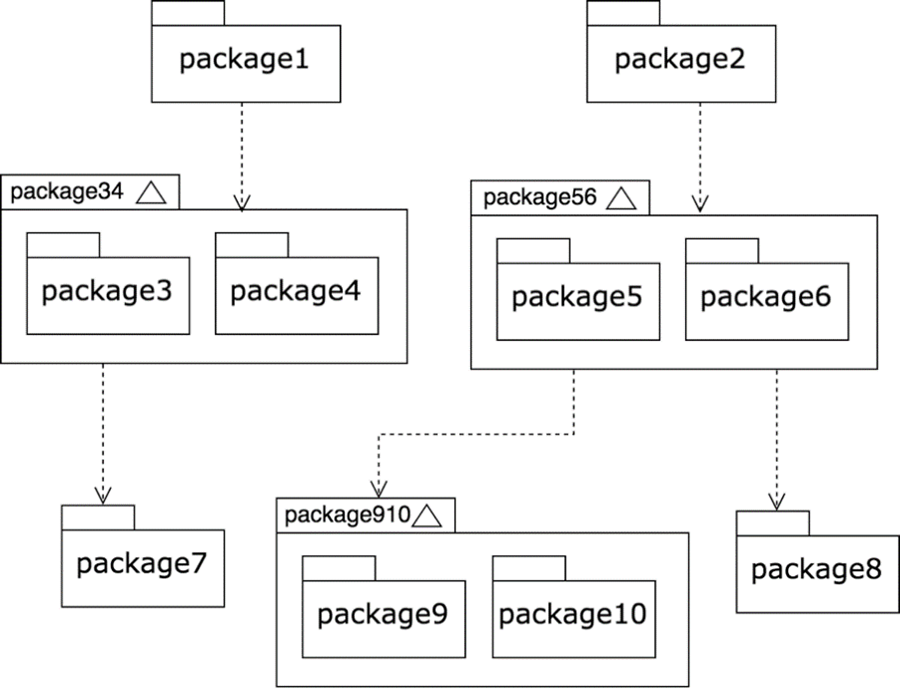
\includegraphics[width=\textwidth]{Figure/Picture3.png}
              \caption{Website ohanaliving.vn}
              \label{fig:ohanaliving}
          \end{figure}
\end{itemize}

\subsection{The importance of this topic}

The demand for accommodation for students and workers has been a persistent and challenging issue for many years, especially with the increasing number of students and workers studying or working far from home nowadays.
Finding satisfactory rental accommodations is difficult due to the rise of fraudulent listings.
Scammers take advantage of renters' vulnerabilities to deceive them into paying deposits or inflate rental prices through intermediaries who sublet at exorbitant rates, making it financially burdensome for many to secure housing.

Providing solutions to the housing issue for workers and students not only improves quality of life but also contributes to the overall socio-economic development of the country.

The ``Accommodation Search Support'' website is created to directly connect renters and landlords without intermediaries, offering affordable fees for listings.
It provides accurate and quick information for renters to find accommodation within desired price ranges and locations.
This platform helps renters find housing without the need for extensive travel to search for rental properties.

Therefore, this topic is not only highly relevant but also holds significant importance for the community, contributing to improving living conditions and reducing difficulties in finding accommodations for students and workers in Vietnam.

\end{document}
